\documentclass[spanish,12pt,a4paper,final,oneside]{book}
\setlength{\parindent}{0pt}
\setlength{\parskip}{0.5em}
\usepackage[spanish]{babel}
\usepackage[utf8]{inputenc}
\usepackage[bottom]{footmisc}
\usepackage[a4paper, total={15cm, 23cm}]{geometry}

\usepackage{longtable}
\setlength{\tabcolsep}{12pt}

\usepackage{amsmath}
\usepackage{amsfonts}
\usepackage{amssymb}

\usepackage{graphicx}
\graphicspath{ {./imagenes/} }

\usepackage[colorlinks]{hyperref}
\hypersetup{colorlinks=true}
\hypersetup{urlcolor=blue}
\usepackage{cleveref}

\usepackage{fancyhdr}
\fancyhf{}
\fancyhead[RE]{\small\scshape\nouppercase{\leftmark}}
\fancyhead[LO]{\small\scshape\nouppercase{\leftmark}}
\fancyhead[LE,RO]{\small\thepage}
\pagestyle{fancy}

\usepackage{authoraftertitle}
\title{Industrialización y \\ transformación digital \\ de la construcción}
\author{Juan Murua Olalde}
\date{11/Marzo/2019}

\begin{document}

\begin{titlepage}

\begin{flushright}
\vspace{2cm}
\begin{Huge}\MyTitle\end{Huge}

\vspace{0.3cm}
{\large BIM (\textit{Building Information Modeling})}

{\large VDC (\textit{Virtual Design and Construction})}

\vspace{1cm}
\MyAuthor

\vspace{1cm}
\MyDate
\\ \today
\\\end{flushright}

\begin{flushleft}
\vspace{3cm}

\textit{``Da información a las personas, y podrán \\tomar decisiones correctas por sí mismas.''}

\vspace{1.5cm}
\textit{``Una herramienta ayuda a hacer el trabajo, pero no hace el trabajo.\\ Es el conocimiento de cómo usar la herramienta lo que hace el trabajo.''}

\begin{footnotesize}(Aprende a utilizar las herramientas adecuadamente, para sacar el máximo provecho de ellas.)\end{footnotesize}

\end{flushleft}

\vfill
\begin{small}
Nota: Una copia .pdf de este manual se puede descargar desde \url{www.susosise.es}
\\Nota: El código fuente y el historial de cambios de este documento se puede obtener en \\ \url{https://bitbucket.org/susosise/industrializacion_y_transformacion_digital_de_la_construccion/commits/}
\end{small}
\begin{flushleft}

\includegraphics[scale=0.3]{CreativeCommons-Attribution-ShareAlike-logo}
\begin{small}\url{https://creativecommons.org/licenses/by-sa/4.0}\end{small}
\end{flushleft}

\end{titlepage}

\hypersetup{linkcolor=black}
\tableofcontents


\chapter{Introducción}

\section{Qué es BIM}

BIM se refiere al manejo de información en la construcción
\\BIM $\rightarrow$  `Building Information Modeling'

La letra clave en BIM es la I de información. Tanto es así que incluso hay quien lo interpreta como `Building Information Management'.

En los últimos tiempos ha surgido otro acrónimo: VDC $\rightarrow$ `Virtual Design and Construction'. Reflejando el hecho de que la `metodología de trabajo BIM' va más allá del mero modelado. E involucra todo el ciclo de vida, desde el diseño inicial hasta la construcción; (e incluso durante la operación y mantenimiento de lo construido). 

En este sentido, la norma ISO19650-1 define BIM como: “uso de una representación digital compartida de un activo construido para facilitar los procesos de diseño, construcción y operación del mismo, y para proporcionar una base confiable para la toma de decisiones.”

La clave de que todo este movimiento haya surgido ahora está en las palabras ``digital'' y ``compartida''. Las nuevas tecnologias digitales (ordenadores y redes) posibilitan manejar información a una escala y de una forma muy distinta a lo que antes era posible con las tecnologias analógicas (papel y teléfono).

Son estas nuevas posibilidades de manejar y compartir información las que están llevando a nuevas formas de trabajar. En todas las fases de vida del activo a construir.

\section{Y eso, ¿cómo se plasma en la práctica?}

BIM es:
\begin{itemize}

\item Un proceso colaborativo, entre todos los participantes.

\item Un proceso que se puede aplicar en todo el ciclo de vida de un activo: diseño, construcción, operación y retirada.

\item Un proceso basado en modelos 3D con información asociada. Modelos que se comparten entre los participantes.  

CDE (Common Data Environment) (Entorno Compartido de Datos)

\begin{small}
nota: Un `modelo BIM' no tiene por qué ser un solo documento (un solo archivo). Normalmente suele estar compuesto por varios y en varios formatos. Se podria decir que un `modelo BIM' es ``toda la información necesaria acerca de algún aspecto del activo a construir, en construcción o construido''.
\end{small}

\begin{small}
nota: Un modelo puede tener variados usos. En función de para qué se vaya a utilizar, se tendrá que modelar de una u otra manera y se tendrán que incorporar al mismo unas u otras informaciones.
\\En cada caso, el cliente (quien paga) es quien sabe qué necesita y qué ha de pedir. Teniendo en cuenta que, como en todo trabajo, el coste va en función de lo que se solicite hacer.
\end{small}

\begin{small}
nota: `Compartido entre los participantes' no significa que todos compartan todo. Cada cual puede tener los documentos de trabajo propios que considere oportuno. Se comparte lo que esté acordado compartir, aquello que es útil a más de un participante y que facilita el desarrollo del proyecto.
\end{small}
\begin{center}
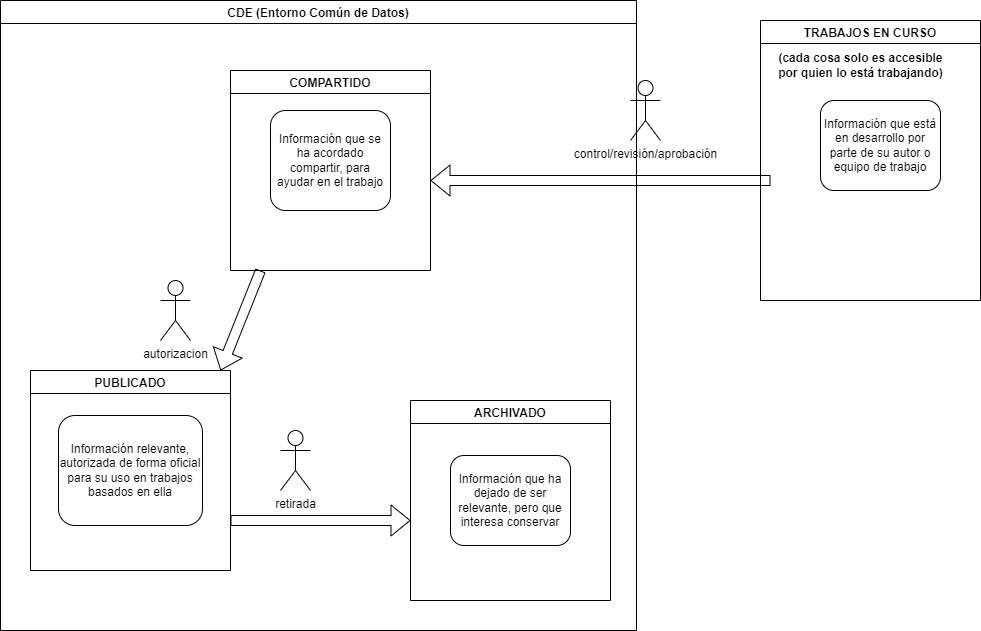
\includegraphics[width=0.8\textwidth]{posibles estados de los documentos trabajando con un CDE}
\end{center}

\item Un proceso donde no se ``dibuja'' al diseñar, sino que se ``construye'' de forma virtual en la pantalla de un ordenador.
\\ Resultando una documentación más rica y precisa. Teniendo menos problemas ``sobrevenidos'' aguas abajo, por ejemplo, en la obra real.

VDC (Virtual Design and Construction) (Diseño y Construcción Virtuales)


\end{itemize}

En resumen: un proceso donde la información circula de forma fluida, allá donde se necesite, cuando se necesite.



\section{Las ventajas de usar BIM}
Básicamente, todas las ventajas de la metodologia BIM provienen de ahorros y mejoras de eficiencia derivadas de la colaboración entre las diversas partes participantes en el proyecto.

Esa colaboración se estructura en torno a un modelo digital compartido. Este modelo no tiene por qué ser un único documento; casi siempre será una colección de documentos (archivos), estructurados de una cierta manera (carpetas, etiquetas,...), en un repositorio (almacén) común.

Trabajar con metodogía BIM consiste en que toda la información relevante se va agregando al modelo según va estando disponible. Y en que este modelo es accesible para todos los participantes. De tal forma que cada participante:
\begin{itemize}
\item Por un lado, se apoya para su trabajo en la información existente en el modelo.
\item Y, por otro lado, va enriqueciendo el modelo con nueva información derivada de su trabajo.
\end{itemize}
Las ventajas de trabajar con metodología BIM se derivan de:
\begin{itemize}
\item evitar repetición de trabajos ya hechos,
\item mejor coordinación de trabajos, 
\item evitar errores por falta de información.
\end{itemize}

\subsubsection{notas para reflexionar\ldots}
Si las ventajas provienen del trabajo colaborativo. Es muy posible que alguien se pregunte por qué se arma ahora tanto revuelo en torno a esto. Si esto es todo lo que es BIM. Bien podria haber existido desde hace tiempo. Solo habria hecho falta tener voluntad de colaborar.

Conceptualmente, BIM podia haberse aplicado hace tiempo. Pero no hubiera sido tan rentable de aplicar como lo es hoy en día. Sin el auxilio de la gran capacidad de manejo de datos de los actuales ordenadores, de los actuales dispositivos móviles (tablets, escaneres 3D, cámaras 360, drones,...) y de las actuales comunicaciones ubicuas (Internet en prácticamente cualquier lugar) hubiera resultado muy costoso compartir de forma ágil la gran cantidad de información presente en cualquier proyecto de construcción. 

\section{VDC (Virtual Design and Construction)}
 
Trabajando con los tradicionales softwares de dibujo CAD, procesadores de texto y hojas de cálculo, cada aspecto del diseño se recoge por separado.

De ahí que estemos acostumbrados a que un estudio de arquitectura o de ingenieria civil realice el diseño base. Luego estudios especializados de estructuras y de instalaciones realicen cada cual diseños detallados de cada disciplina. Y, al final, la constructora, con sus subcontratas, realicen las adaptaciones que vayan siendo necesarias durante la construcción de lo diseñado.

Cada actor participante realizando su parte y pasando el testigo al siguiente.

Sin embargo, los actuales softwares BIM de modelado, simulación y gestión permiten ir más allá y ``construir'' de forma virtual en lugar de solo ``dibujar y diseñar''. Los modelos digitales elaborados con ellos recogen de forma coherente y detallada
\begin{itemize}
\item tanto los requisitos (cómo se van a satisfacer los usos a los que está destinado lo que se va a construir), 
\item como la forma (la geometria de lo que se va a construir), 
\item como el proceso constructivo (cómo, cuándo y con qué se va a construir).
\end{itemize}

Estos modelos digitales, modelos BIM, permiten involucrarse e interactuar con la futura construcción a un nivel de profundidad imposible de conseguir trabajando solo con documentos textuales y con dibujos 2D o incluso 3D.

Trabajar con esos modelos digitales virtuales es un poco como volver a las épocas de los maestros constructores, donde el diseño de la obra estaba íntimamente ligado a su construcción real.

De ahí que haya surgido el acrónimo VDC: ``Virtual Design and Construction''. Y que comience a verse la conveniencia de que todos los actores involucrados participen desde el principio y conjuntamente en ese proceso de diseño y construcción. 

Esta nueva forma de trabajar ofrece toda una serie de ventajas:
\begin{enumerate}

\item En la fase de diseño,
\begin{itemize}

\item Permite trabajar de forma conjunta a todas las disciplinas. Superponiendo los diseños de cada una de ellas. Atendiendo y coordinando las necesidades de todas ellas. De tal forma que se llega a un diseño construible, sin errores ni interferencias graves, un diseño mejor optimizado y más sencillo de llevar a la práctica.

\item Cuesta poco probar diversas alternativas sobre un modelo virtual (“los pixeles son mas baratos que los ladrillos”). Además, permiten realizar estimaciones y simulaciones para analizar la adecuación o el rendimiento de cada una de esas alternativas.

\end{itemize}

\item En la fase de construcción propiamente dicha, 
\begin{itemize}

\item Permiten ir comprobando el progreso de la construcción, superponiendolo y comparándolo con lo previsto en los modelos.

\item Los posibles incidentes que vayan surgiendo se localizan sobre el modelo y se transmiten a quien corresponda. De tal forma que llegan a quien deban llegar no solo con más rapidez, sino también con mayor detalle y precisión.  

\item El modelo virtual va evolucionando y enriqueciéndose a medida que se va ejecutando la construcción física. De tal forma que, al terminar la construcción, termina recogiendo de manera fiel lo construido (modelo ``as built'').
\end{itemize}

\item En la fase de operacion y mantenimiento,
\begin{itemize}

\item En cada intervención de reparación, remodelación o ampliación, toda la información recogida en los modelos es de inestimable ayuda. Información tal como, por ejemplo: detalles constructivos internos, trazados de conducciones ocultas, hojas de especificaciones de equipos, datos de los proveedores de los distintos elementos, etc.
\\nota: La nueva información fruto de la intervención también ha de quedar recogida en el modelo correspondiente

\item A la hora de establecer calendarios y recordatorios de trabajos son de gran ayuda informaciones tales como, por ejemplo: fechas de expiración de garantias, plazos de revisiones periódicas obligatorias, etc. 

\item La información gráfica del modelo es muy útil para dar soporte a los interfaces HMI del sistema de control y gestión. Permitiendo visualizar con precisión la ubicación de los sensores de donde proceden los datos o de los actuadores que se van a activar con los comandos.


\end{itemize}

\end{enumerate}

\chapter{BIM en la fase de diseño}

\section{Documentación previa}
Se incorpora al modelo BIM información acerca del terreno y de las construcciones existentes. 

Parte de esta información se puede obtner de forma más o menos automatizada utilizando tecnologias tales como la fotogrametria o los escaneres LIDAR. Con instrumentos basados en tierra (precisión de milimetros) o desplegados en drones (precisión de centímetros).

Las ‘nubes de puntos’ generadas por estos instrumentos pueden servir como base sobre la que realizar mediciones o sobre la que apoyarse al diseñar la nueva construcción.

\section{Diseño conceptual y arquitectural}
Se aprovecha el modelado 3D para realizar estudios preliminares de formas y espacios.

Con el modelado 3D, se diseña la construcción, elaborando un modelo más o menos detallado del mismo. Este modelo de la construcción se irá refinando/ampliando/completando en sucesivas etapas de diseño.

Se va incorporando al modelo la correspondiente información adicional para obtener listados de superficies o volúmenes, presupuestos preliminares, análisis de cumplimiento de normativas, análisis energéticos, etc.

Se aprovecha el modelo geométrico para elaborar renderizados artísticos publicitarios y de presentación al cliente.

\section{Cálculos estructurales}
Apoyándose en el diseño inicial, se dimensionan y se calculan las estructuras de soporte. Llegando a detallar todos los aspectos relevantes de las mismas.

En este proceso, es posible que se deban realizar cambios en el diseño. Es decir, es importante disponer un intercambio bidireccional fluido de datos entre el modelo de diseño y el modelo de cálculo.

\section{Instalaciones y equipamientos}
Se incorpora al modelo BIM el detalle de los equipamientos: fontaneria, electricidad, aire acondicionado, calefacción, iluminación, automatismos, etc.

Aquí es quizás donde son más claras las ventajas aportadas por la metodología BIM. Al coordinar las distintas disciplinas entre sí, se obtiene un diseño de instalaciones más limpio, coherente y sin interferencias.

Elaborar un detallado modelo 3D digital de las instalaciones facilita su optimización y la posibilidad de prefabricar partes de las mismas fuera de la obra.

En el aspecto geométrico, no es necesario que cada componente sea exactamente tal y como es en la realidad. Pero sí es importante que incluya sus detalles relevantes: la ubicación y dimensiones de las tomas de fluidos y racores de paso de cables, ubicaciones de los paneles de control, espacios a dejar libres para acceso, etc. De esta forma, se podrán ubicar esos componentes correctamente respecto del resto de elementos dentro de la instalación.

Además, las herramientas BIM que trabajan estas disciplinas suelen incorporar módulos de cálculo y dimensionamiento, en aspectos tales como: presiones de suministro, caudales de aire, pérdidas de calor, potencias consumidas, secciones de cable, caidas de tensión, etc. Para esto, es importante que los componentes individuales incorporados al modelo BIM incluyan toda la información relevante acerca de sus parámetros nominales de funcionamiento.

\section{Análisis de rendimiento}
Es lo que suele denominar 6D. Se utiliza el modelo BIM para analizar cómo se comportará la construcción en aspectos tales como:
\begin{itemize}
\item consumo de energia,
\item iluminación natural de espacios,
\item tráfico/circulación (de vehículos, de personas,...),
\item impacto visual y medioambiental,
\item etc.
\end{itemize}

\chapter{BIM en la fase de construcción}

\section{Planificación}
Es lo que se suele denominar 4D. 

Se incorpora al modelo BIM información temporal acerca de cuándo prevé demoler o construir cada una de las partes de la obra.

Esto permite hacer previsiones y elaborar paquetes de construcción para planificar las distintas fases y las tareas concretas a ejecutar en cada una.

\section{Estimación de costos}
Es lo que se suele denominar 5D.

Se utiliza el modelo BIM para estimar listas de materiales, realizar mediciones virtuales de operaciones a realizar,... Para luego tratarlas y completarlas en un programa de gestión de costes.

En este sentido, cobran importancia estándares de codificacion tales como Omniclass. Uniclass, MasterFormat,... Para facilitar la identificación homogénea de cada una de las partidas de gastos. 

\section{Logística}
Se aprovecha el modelo (3D) y la información temporal (4D) para planificar dónde y cuándo se ha de entregar cada material en la obra.

Esto permite también prefabricar fuera de la obra. Coordinando la entrega en obra de cada parte prefabricada cuando vaya a ser instalada.

\section{Gestión del trabajo}
Se aprovecha la información temporal y los paquetes de trabajo elaborados durante su planificación:
\begin{itemize}
\item Para lanzar partes de tareas a realizar.
\item Para recoger partes de trabajos realizados.
\end{itemize}

Los modelos BIM y la información asociada a los mismos, son de gran utilidad durante la ejecución de los trabajos:
\begin{itemize}
\item No solo por la referencia visual o la posibilidad de tener siempre a mano toda la información (dimensiones, calidades, modelos,...). En dispositivos tales como pantallas táctiles, tablets o móviles.
\item Sino también a la hora de ubicar con precisión puntos significativos referenciados al modelo. Con dispositivos tales como estaciones topográficas o sistemas georeferenciales.
\end{itemize}

Además, cualquier duda que surja en la obra, se puede resolver de forma más eficiente si se referencia directamente, sobre el modelo correspondiente, al punto conflictivo involucrado.

Y las inspecciones en obra se facilitan en gran medida al:
\begin{itemize}
\item Referenciar sobre el modelo fotografias u otras evidencias recogidas durante la inspección.
\item Detectar errores automáticamente, escaneando lo construido (fotogrametria, LIDAR,...) y comparandolo con lo previsto construir (el modelo 3D).
\end{itemize}

Si el trabajo se realiza siguiendo la metodología BIM, el modelo digital se va actualizando progresivamente. En todo momento se va reflejando en él el estado real de la obra. Cada vez con mayor detalle, incorporando de forma continua información sobre los componentes reales que se van construyendo/instalando.

\subsubsection{notas para reflexionar:}
Es mucho más fácil corregir/ajustar sobre un modelo digital que sobre una construcción física. De ahí la importancia de modelo BIM, modelo virtual, ``gemelo digital'' (digital twin) de la construcción real.

Cuando se detecta cualquier discrepancia entre el diseño/planificación previsto y lo construido/ejecutado realmente. Es importante incorporar esa información al modelo inmediatamente, en el mismo momento en que se detecta. Así se puede reaccionar con agilidad y se evita la propagación de problemas.

Con una comunicación fluida entre todas las partes, actuaciones posteriores podrán tener en cuenta los cambios sobrevenidos en las actuaciones ya ejecutadas. Es decir, se podrán ajustar con tiempo las posteriores actuaciones, rediseñándolas sobre el modelo digital.

\chapter{BIM en la fase de operación y mantenimiento}

\section{Información detallada sobre el edificio, tal y como ha sido construido}
Es lo que se suele denominar 7D.

Al terminar una obra siguiendo la metodologia BIM,  el modelo digital refleja fielmente lo construido y lleva incorporada toda la documentación asociada. Es lo que se va a entregar al cliente, el modelo final ``as built''.

nota: ``as built'' presupone que, a medida que se ha ido construyendo, se han ido incorporando al modelo digital no solo las variaciones constructivas, sino también todo tipo de detalles importantes. Por ejemplo, los datos relevantes de todos y cada uno de los elementos instalados:  fabricante, modelo, número de serie, proveedor, garantia, manual de funcionamiento, manual de mantenimiento,...

nota: esta información adicional puede ir incorporada directamente en las propiedades de los elementos del modelo, o puede ir en forma de archivos externos (catálogos, hojas de especificaciones,...).

\section{Mantenimiento, gestión de cambios}
Al igual que era importante actualizar el modelo e ir documentando cambios y detalles a medida que se iba construyendo\ldots 
\\ \ldots Es igual de importante seguir actualizando el modelo a medida que se realicen intervenciones de mantenimiento/remodelación. A lo largo de toda su vida útil.

\chapter{Los diferentes ``usos BIM''}
Uso BIM $\rightarrow$ cada uno de aspectos en los que puede resultar útil trabajar con metodología BIM.


\section{Consideraciones previas:}

Por `modelo' se entiende todo el conjunto de archivos y documentos que sean necesarios para contener la información a suministrar.
\\{\footnotesize Se suele llamar también ``modelo'' a cada archivo generado en un software de modelado BIM. En ese sentido, el `modelo' puede contener múltiples ``modelos'' y otros documentos.}

Por `disciplinas' se entiende los diversos aspectos de la construcción: terreno/ubicación, estructuras, edificios, acabados, instalaciones eléctricas, instalaciones de fontanería, instalaciones HVAC,...

Por `nivel de definición suficiente' se entiende el LOD/LOI que se establezca en el BEP para cada uno de los tipos de elementos en el modelo, a lo largo de las diversas fases de la construcción y para cada uno de los usos BIM contemplados para estos.




\subsubsection{Grados de madurez en la aplicación de la metodología de trabajo BIM:}

\begin{description}

\item[pre-BIM:] Cada disciplina elabora su propio modelo, de forma independiente. Y, generalmente los entregables suelen ser los tradicionales: planos, listados, informes,\ldots
\\Es posible que se contemple algún tipo de intercambio puntual de modelos a efectos de facilitar a alguna disciplina su trabajo al poderse apoyar, en algún momento puntual, en algún modelo previo de alguna otra disciplina.

\item[BIM básico:] Se consolida un modelo federado entre disciplinas, para resolver interferencias de diseño entre ellas.
\\Se requiere la figura de un coordinador BIM que vele por la coherencia de los modelos parciales a federar.
\\Se requiere acordar las disciplinas que se van a incluir en la federación. Preparando una matriz de qué modelos se van a comprobar contra cuales. Indicando en cada cruce el margen de aproximación a aplicar para considerar o no algo como interferencia a resolver.

\item[BIM:] Se utiliza un modelo común compartido, para facilitar y coordinar trabajos entre disciplinas. Ello no quita para que cada participante pueda tener además su propia información privada de trabajo en sus sistemas particulares. Pero toda la información relevante está en un único sitio.
\\Se requiere la figura de un coordinador BIM que vele por la coherencia e interoperabilidad de la información compartida.
\\Se requiere acordar el soporte y las normas comunes de modelado necesarias para la interoperabilidad fluida entre todas las partes implicadas.

\end{description}

\section{Un resumen rápido}
Básicamente, podriamos distinguir tres objetivos cuando se plantea trabajar con metodologia BIM:
\begin{itemize}
\item Modelar para documentar.
\item Modelar para analizar y diseñar.
\item Modelar para construir.
\end{itemize}

Cada uno de estos objetivos requiere una forma diferente de abordar el modelado, de incorporar información a los modelos, de coordinarse entre las distintas partes que trabajan en el proyecto,... Y, obviamente, tiene también un coste de trabajo diferente.


\section{Detalle de algunos usos BIM}
Uso BIM $\rightarrow$ cada uno de aspectos en los que puede resultar útil trabajar con metodología BIM.

Como se ha comentado, cada uso tiene unas ciertas implicaciones en el modelo a elaborar. A grandes rasgos:

\begin{itemize}

\item Utilizar el modelo \textbf{para definir el proyecto preliminar}.
\\Se requiere definir los principales volúmenes y elementos con un nivel de definición suficiente para hacerse una idea de cómo será la construcción. Pero sin ser suficiente para ejecutarla.
\\Se requiere definir los elementos con un nivel de definición suficiente para realizar mediciones aproximadas y extraer cantidades como para elaborar un primer presupuesto orientativo.

\item Utilizar el modelo \textbf{para elaborar imágenes o videos 3D de presentación} o de promoción de la construcción.
\\Se requiere enriquecer el modelo con los materiales (texturas) y detalles adecuados para su representación fotorealista.
\\Para las imágenes, se han de acordar las partes de la construcción que se desean mostrar y los tamaños/soportes en los que se van a distribuir.
\\Para los videos, se ha de acordar el propósito de los mismos y las resoluciones/soportes en que se van a distribuir.

\item Utilizar el modelo \textbf{para elaborar la documentación} gráfica de la construcción: planos, vistas, detalles constructivos,\ldots 
\\Se requiere elaborar la geometría de los elementos con un nivel de definición suficiente como para elaborar la documentación requerida. Sin perder de vista que los modeladores BIM  permiten también enriquecer con detalles 2D directamente en los documentos que así lo requieran. Es decir, no es necesario diseñar absolutamente todo con total realismo en el 3D.

\item Utilizar el modelo \textbf{para realizar controles de interferencias} en el diseño de los diversos sistemas de diversas disciplinas.
\\Se requiere acordar unas referencias geométricas precisas, para que todos los modelos de cada disciplina estén referenciados a ellas, de tal forma que se puedan superponer entre sí.
\\Se ha de acordar una 'matriz de interferencias' (cuales modelos se comprobarán contra cuales otros) y el concepto de ``proximidad'' (x cm, x mm, x\ldots) a aplicar para según qué tipos de elemento.
\\Y, obviamente, la geometría 3D de cada elemento se ha de modelar de acorde a las dimensiones reales del mismo (por lo menos en cuanto a su ``envolvente'' exterior) y cada elemento se ha de posicionar con la precisión adecuada.

\item Utilizar el modelo \textbf{para realizar mediciones y elaborar presupuestos} detallados de la construcción.
\\Se requiere modelar cada elemento tal y como se va a construir. Para poder ubicar cada elemento en el apartado de clasificación correspondiente según el sistema de clasificación que se vaya a emplear. \\Y se han de enriquecer con las propiedades pertinentes para poderlos clasificar/agrupar; y también con toda aquella información que facilite el metraje. 
 
\item Utilizar el modelo \textbf{para realizar una planificación temporal} de la construcción.
\\Se requiere modelar cada elemento tal y como se va a construir. Para poder ubicar cada elemento dentro de la fase de construcción que le corresponda.
\\Y se han de enriquecer con las propiedades pertinentes para saber cuándo se va a ejecutar cada uno.

\item Utilizar el modelo \textbf{para realizar cálculo, análisis y dimensionamiento estructural}.
\\Se requiere detallar y enriquecer los elementos del modelo con información relativa a su comportamiento estructural, tanto de forma individual como en relación a los elementos adyacentes con los que interactúa.

\item Utilizar el modelo \textbf{para realizar cálculo, análisis y dimensionamiento de instalaciones eléctricas}.
\\Se requiere detallar y enriquecer los elementos del modelo relativos a las propias instalaciones con información relativa a su comportamiento eléctrico, tanto de forma individual como en relación a los elementos adyacentes con los que interactúa.

\item Utilizar el modelo \textbf{para realizar cálculo, análisis y dimensionamiento de instalaciones de fontanería, calefacción y/o aire acondicionado}.
\\Se requiere detallar y enriquecer los elementos del modelo relativos a las propias instalaciones con información relativa a su comportamiento hidrostático, neumático o hidráulico, según corresponda; tanto de forma individual como en relación a los elementos adyacentes con los que interactúa.

\item Utilizar el modelo \textbf{para realizar cálculo, análisis y dimensionamiento de iluminación} de espacios.
\\Se requiere enriquecer el modelo fijando la ubicación/orientación real de la construcción. Para estimar y estudiar la iluminación solar natural a lo largo del año.
\\Se requiere enriquecer el modelo con información de desempeño real de los diversos sistemas de iluminación artificial que se hayan incluido en el mismo.

\item Utilizar el modelo \textbf{para realizar análisis y optimización energética}.
\\Se requiere enriquecer el modelo fijando la ubicación/orientación real de la construcción. Para estimar la iluminación solar natural y los principales parámetros climáticos a lo largo del año.
\\Se requiere indicar las distintas zonas de la construcción y cual es el uso al que está destinada cada una.
\\Se requiere detallar y enriquecer los elementos del modelo con información relativa a aspectos tales como: transmitancia de calor, afectación por exposición solar, puentes térmicos entre elementos, rendimiento en transporte/transformación de energia, etc.

\item Utilizar el modelo \textbf{para realizar análisis y optimización de circulación de personas o vehículos}.
\\Se requiere detallar y enriquecer el modelo con información acerca de aspectos tales como: usos previstos para los diversos espacios, las áreas de circulación previstas entre ellos, las áreas de exclusión, las dimensiones mínimas de estas según normativas, los flujos de personas o de vehículos esperados, etc.

\item Ejecutar la obra utilizando el modelo \textbf{para guiar, coordinar y comprobar los trabajos}.
\\Se aplican los anteriores usos de realizar mediciones/presupuestos y de realizar planificación temporal.
\\Se requiere una codificación/identificación clara de todas y cada una de las zonas/partes de la construcción. De tal forma que, con esos códigos, se puedan referenciar las órdenes de trabajo, las peticiones de información adicional o aclaraciones, las recepciones de material, los reportes de incidencias, los partes de seguimiento, etc.
\\Se requiere de una georeferenciación adecuada, de tal forma que se puedan trasladar puntos significativos del modelo sobre la obra real y se puedan contrastar mediciones sobre la obra real contra el modelo.

\item Ejecutar la obra utilizando prefabricación.
\\Se aplican los tres anteriores usos de realizar mediciones/presupuestos, de realizar planificación temporal y de guiar/coordinar/comprobar trabajos.
\\Se requiere detallar el modelo subdividiendolo en los paquetes necesarios.
\\Cada paquete requiere su propio submodelo, con el nivel de definición adecuado para su fabricación fuera de la obra y su posterior montaje en la misma.
\\Se requiere enriquecer el modelo con la información necesaria para coordinar la logística de suministro de cada paquete en el momento y lugar adecuados.

\item Utilizar el modelo \textbf{para registrar con detalle lo realizado y tener así una documentación adecuada para la posterior gestión y mantenimiento de la construcción} una vez terminada esta.
\\Se aplica el anterior uso de guiar/coordinar/comprobar trabajos.
\\Se requiere ir enriqueciendo el modelo a medida que avanza la construcción. Recogiendo lo realmente ejecutado (modelo “as build”). Recogiendo toda la información relevante sobre cada elemento (marca, modelo, número de serie, proveedor, garantia, manual técnico,\ldots). Además de todo tipo de documentos e información adiccional que pueda resultar relevante (catálogos, manuales, hojas de especificaciones,\ldots)
\\Aunque parezca de Perogrullo, es importante tener en cuenta que toda esa información se tendrá que continuar enriqueciendo a medida que se van realizando posteriores intervenciones de mantenimiento sobre la construcción, a lo largo de toda su vida útil. 

\item etc.

\end{itemize}



\chapter{Normativas, contratos, requisitos, estandares,\ldots}
Hay algunos documentos y cláusulas contractuales específicos de la forma de trabajar BIM.

\section{BEP (Bim Execution Plan),\\para qué se va a usar BIM en este proyecto}
Este documento recoge los usos que se le van a dar al modelo BIM a lo largo del proyecto.

Como se ha visto en capítulos anteriores, la forma de trabajar BIM se puede utilizar en todas las etapas del ciclo de vida de cualquier edificio. Pero como BIM está aún en sus inicios, en estos momentos se suele utilizar solo de forma parcial. De ahí la necesidad de este documento BEP. Para dejar claro desde el principio dónde se va a usar BIM y dónde no; en qué fases se va a requerir trabajar sobre un modelo digital y en cuales no; que información ha de incluirse en dicho modelo y cual no; qué información ha de compartirse y cómo se ha de concretar esa compartición; etc.

Una vez BIM sea la forma habitual de trabajar, probablemente el documento BEP será innecesario.  Pero en estos momentos (año 2019), es el documento cuya existencia o inexistencia suele ser un buen indicador de si estamos ante un proyecto donde realmente se nos va a pedir trabajar de forma BIM. O ante un proyecto donde solo se está usando el acrónimo BIM porque ``está de moda''; pero donde, en realidad, se va a trabajar ``como siempre''.

nota: Ver la norma ISO 19650, en el apartado \ref{estandarISO19650}; y algunas cuestiones a recoger en el BEP, en el capítulo \ref{cuestionesEnElBEP}. Muchas de las cuestiones reflejadas en los BEP ahora, es muy posible que en un futuro se recojan en los documentos prescritos por la norma ISO 19650.

\section{Nomenclatura, códigos de clasificación y códigos identificadores}
Adoptar un sistema de nomenclatura acordado para la identificación de cada parte del proyecto. Es algo que ya se viene haciendo desde antes de BIM.

Pero con ``BIM'' cobra una especial relevancia: al trabajar todos los participantes sobre un modelo digital común,  es importante utilizar el mismo vocabulario para identificar y referirse a cada parte del modelo.

En ese sentido, es también importante asignar códigos de clasificación estandarizados a las distintas partes. Para así facilitar la elaboración de listas agrupadas; como, por ejemplo, listas de materiales y presupuestos.

Prácticamente todos los modeladores BIM suelen asignar códigos identificadores únicos para cada entidad del modelo. De esta forma se facilita el referenciarlas al relacionarlas con información adicional, al buscar la vista correspondiente en las que se pueden ver, al realizar consultas o comunicar incidencias sobre ellas, etc.


\section{LOD (Level Of Development, Level of Detail)\\LOIN (Level Of Information Need)\\NDI (Nivel de Información),\\el nivel de definición de elementos necesario para cada uso que se va a hacer de BIM}
Este concepto recoge el nivel de definición necesario para cada elemento, según cada uso que se le vaya a dar al modelo BIM durante el proyecto.

Esta definición puede darse en tres aspectos principalmente:
\begin{description}
\item[geometria]: lo que debe verse en las representaciones gráficas del elemento.
\item[información]: lo que se ha de indicar en las propiedades del elemento.
\item[ficheros]: datos complementarios en archivos externos, bien enlazados o bien sin enlazar a elementos del modelo. (por ejemplo un catálogo o una hoja de especificaciones del fabricante del elemento) 
\end{description}

El modelo digital (la M de BIM) del edificio a construir (la B de BIM) puede detallarse más o menos (la I de BIM).

El modelado tiene necesidades diferentes según el uso que se le vaya a dar, por ejemplo, para:
\begin{itemize} 
\item obtener imágenes 3D del edificio, 
\item realizar mediciones y elaborar presupuestos, 
\item guiar a los operarios o para elaborar instrucciones de montaje.
\end{itemize} 

En el primer caso, se ha de prestar especial especial atención a los materiales y al aspecto externo de lo modelado. 

En el segundo caso, se ha de prestar especial atención a la exactitud de medidas y a la correcta identificación de todos y cada uno de los componentes de la construcción. 

En el tercer caso, se ha prestar especial atención a la secuencia de operaciones y a la representación gráfica de los detalles que afectan a cada operación.

\vspace{0.5cm}
Algunos ejemplos ilustrativos puede encontrarse en
\\ \url{https://bimforum.org/lod/}
\\ \url{https://www.bimnd.es/lod-la-metodologia-bim/}
\\ \url{https://planbim.cl/biblioteca/documentos-mide/}


\section{CDE (Common Data Environment), la plataforma concreta de hardware/software sobre la que se va a compartir información}

Obviamente, poca colaboración habrá si cada participante usa solo sus propias herramientas y estas no son compatibles entre sí.

De ahí la importancia de disponer de un comité dentro del proyecto, donde acordar las tecnologias a utilizar. En este comité suelen estar representadas todas las partes participantes en la construcción.

Cada participante es libre de utilizar la tecnologia que desee en sus documentos internos de trabajo. Pero ha de utilizar lo que el comité acuerde en todos aquellos documentos compartidos de uso común.

Es importante que la infraestructura CDE elegida para depositar archivos tenga capacidades para administrar usuarios/equipos/permisos. Esta capacidad de administración facilitará compartir lo que se ha de compartir con quien se ha de compartir.

Es importante que la infraestructura CDE elegida para depositar archivos tenga capacidades para gestionar estados y versiones. La capacidad de gestionar estados facilitará saber que documentos son ``trabajo en curso'' (WIP, Work In Progress) (solo visibles para el equipo que los está trabajando), cuales están ``compartidos'' (conocidos por más de un equipo), cuales ``publicados'' (aprobados para ser utilizados en la construcción), cuales ``archivados'' (retirados y conservados como histórico),\ldots La capacidad de gestionar versiones es importante para saber qué se ha cambiado cuándo y por quien.


\section{Estandares impulsados por buildingSMART}
buildingSMART es una organización internacional, abierta, neutral y sin ánimo de lucro. Dedicada a impulsar estándares en el campo de la construcción.

\url{https://www.buildingsmart.org/}
\\ \url{https://technical.buildingsmart.org/}
\\ \url{https://forums.buildingsmart.org/}

\subsection{IDM (Information Delivery Manuals)}
Los IDM marcan estándares acerca de procesos empresariales de intercambio de información, y de requisitos de datos en dichos intercambios.

Estos mapas de procesos suelen estar escritos en BPMN (Business Process Modeling Notation), a veces con algunas partes escritas en DMN (Decision Model and Notation).

La lista de casos de uso que se han definido hasta ahora, se puede consultar en: \url{https://technical.buildingsmart.org/standards/information-delivery-manual/idm-database/}

Existe también un servicio que ayuda a desarrollar un IDM para un determinado caso de uso concreto: \url{https://ucm.buildingsmart.org/}

Este estándar se ha elevado a nivel de norma ISO, en la ISO 29481-1:2010 e ISO 29481-2



\subsection{IFC schema (Industry Foundation Classes)}
El esquema IFC marca un estándar acerca de cómo representar la información intercambiada en un proceso de construcción.

Permite obtener una copia restringida del modelo digital nativo original, en un formato estándar que cualquiera pueda leer. La idea es poder capturar un momento del proyecto; para compartirlo con otros participantes, aunque estos estén utilizando distintos softwares de trabajo. 

Los detalles técnicos de cada versión del estandar publicada hasta ahora se pueden consultar en: \url{https://technical.buildingsmart.org/standards/ifc/ifc-schema-specifications/}

Este estándar se ha elevado a nivel de norma ISO, en la ISO 16739-1:2018

nota: más información sobre el esquema IFC en el documento \url{https://susosise.es/documentos/El_estandar_IFC.pdf}


\subsubsection{MVD (Model View Definitions)}
Una vista MVD es lo que realmente nos intercambiamos cuando decimos que "nos intercambiamos un IFC". Cada vista MVD es un subconjunto del esquema IFC, adecuado de forma específica para un determinado uso concreto.

La lista de vistas MVDs que se han definido hasta ahora, se puede consultar en: \url{https://technical.buildingsmart.org/standards/ifc/mvd/mvd-database/}

\subsubsection{IDS (Information Delivery Specifications)}
Como los MVDs han resultado un tanto confusos de comprender e implementar, hay una iniciativa para sustituirlos con IDSs.

\url{https://technical.buildingsmart.org/projects/information-delivery-specification-ids/}


\subsection{bSDD (buildingSmart Data Dictionary)}
El diccionario bSDD contiene estandares de terminología; para referirnos a los distintos aspectos contemplados en IFC y otros estándares, en distintos idiomas.
\\Dentro de él están contempladas todas las entidades, propiedades y PSets de IFC. Así como también otros recursos de otros estándares relacionados con la construcción.
\\ \url{https://technical.buildingsmart.org/services/bsdd/}

Es un servicio, al que se puede acceder libremente a través de una API de programación. Los detalles técnicos acerca de esta API se pueden consultar en: \url{https://github.com/buildingSMART/bSDD/tree/master/2020%20prototype}


\subsection{BCF, ({\small BIM} Collaboration Format)}
BCF es un estándar que especifica la información y los protocolos de comunicación a emplear para intercambiarse avisos, preguntas e incidencias, entre diferentes participantes en un proyecto de construcción. 

Los detalles técnicos acerca de comunicación vía archivos XML se pueden consultar en: \url{https://github.com/BuildingSMART/BCF-XML}

Los detalles técnicos acerca de comunicación vía servicios Web RESTfull se pueden consultar en: \url{https://github.com/BuildingSMART/BCF-API}


\section{El estandar ISO 19650} \label{estandarISO19650}

Esta norma estandariza la información exigible en cualquier construcción. Con vistas a garantizar una colaboración fluida a lo largo de todo el proceso.

\subsection{OIR, PIR : intereses generales de cada una de las partes} 
OIR (Organizational Information Requirements): requisitos de información de la organización, relativos a sus objetivos.

PIR (Project Information Requirements): requisitos de información del proyecto, relativos a su desarrollo.

\subsection{AIR, EIR : a la hora de cerrar un acuerdo o contrato}
AIR (Asset Information Requirements): requisitos de información del activo, relativos a su operación.

EIR (Exchange Information Requirements): requisitos de intercambio de información entre las partes sujetas a una contratación.

\subsection{PIM, AIM : información a elaborar y entregar}
PIM (Project Information Model): modelo de información del proyecto, relacionado con la fase de desarrollo.

AIM (Asset Information Model): modelo de información del activo construido, relacionado con la fase de operación y mantenimiento del mismo.

\section{Diagrama resumen de flujos de información}
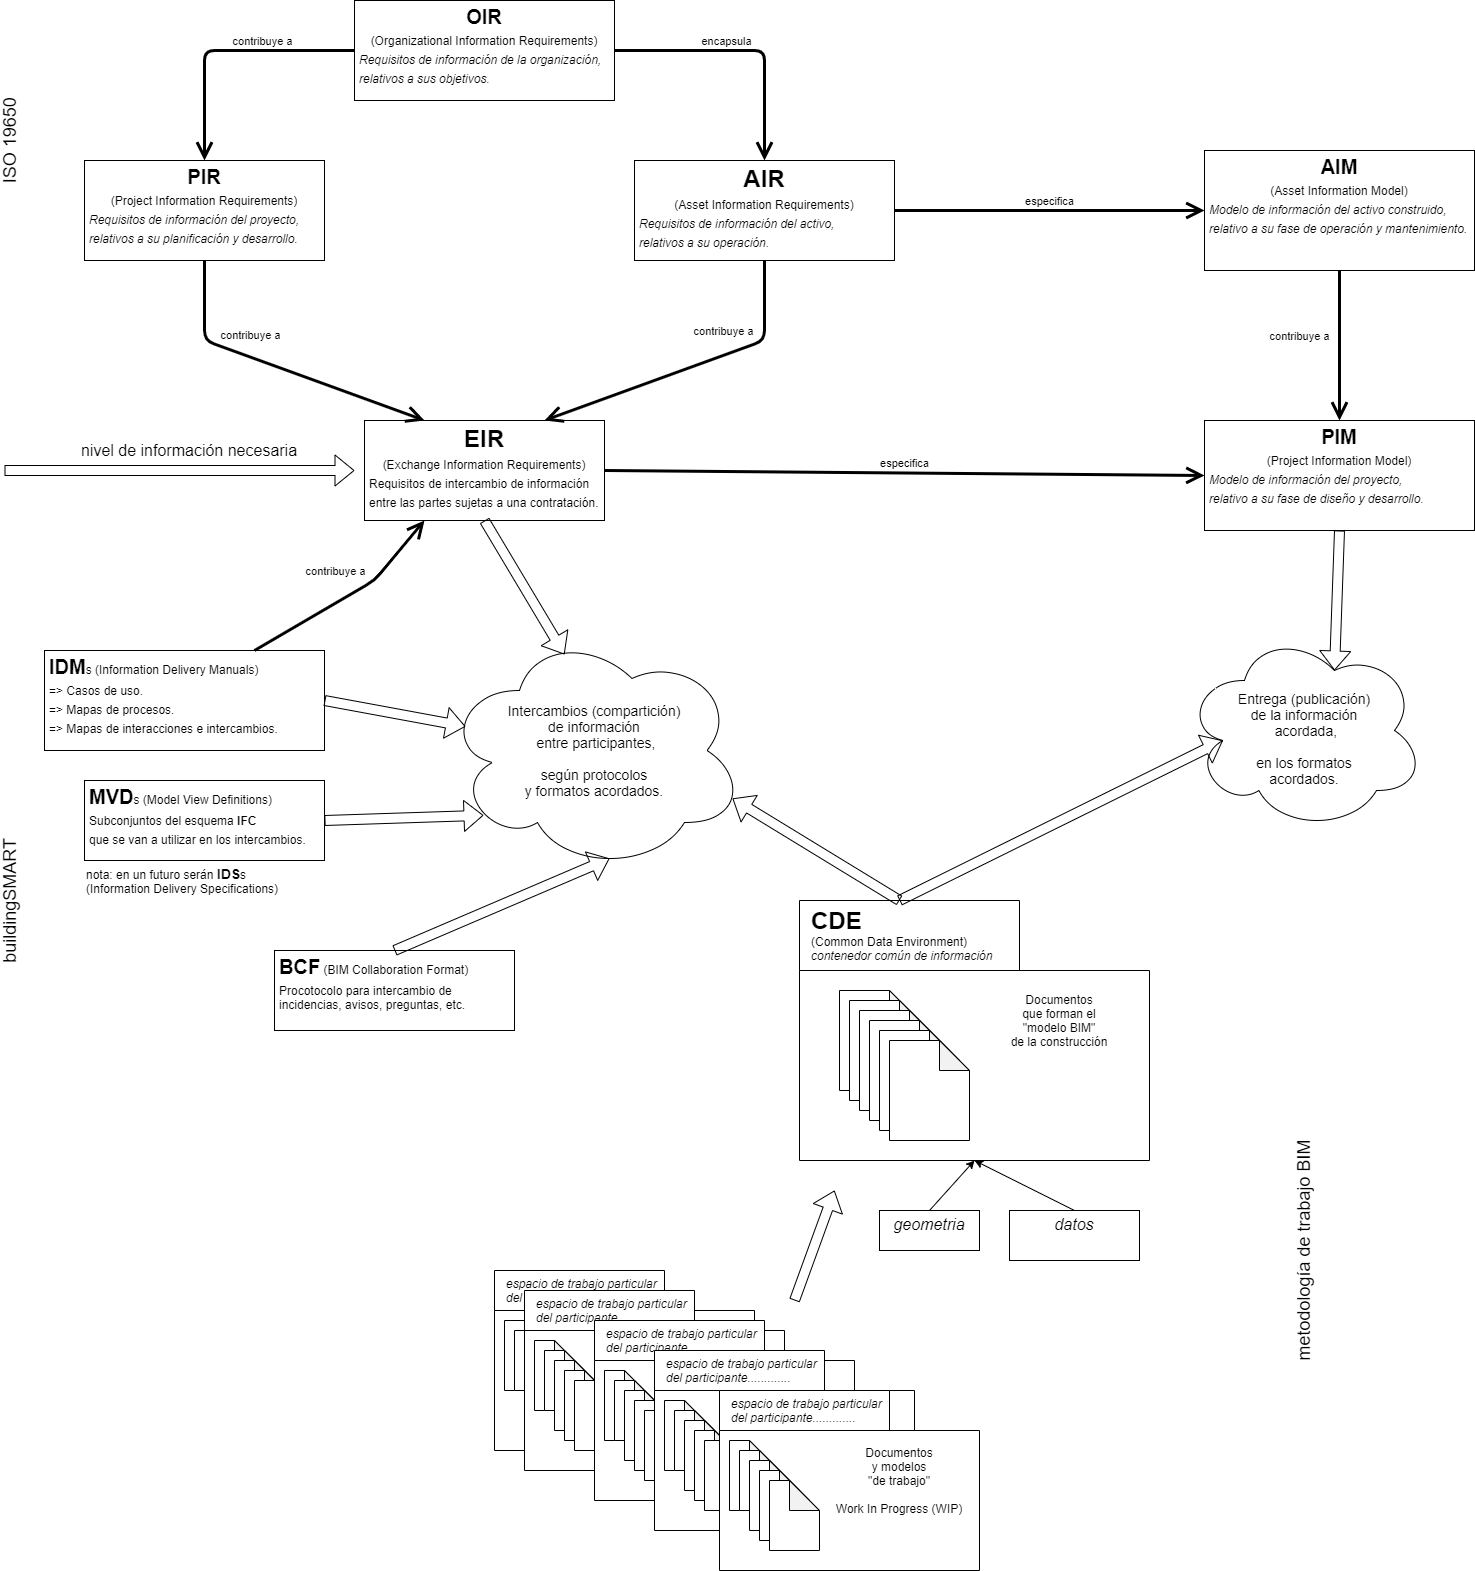
\includegraphics[width=1.2\textwidth]{Flujos de informacion en la construccion BIM}

{\footnotesize  \url{https://www.susosise.es/documentos/Flujos\_de\_informacion\_en\_la\_construccion\_BIM.png}}

\section{(Algunos) enlaces ilustrativos}
BIM está en plena época de definición de formas de trabajar y de los estándares que posibiliten ese trabajo colaborativo entre los diferentes actores implicados. El panorama está cambiando continuamente, según van perfilando necesidades y se van adoptando consensos.

\url{https://www.buildingsmart.org/standards/bsi-standards/}
\\ \url{https://planbim.cl/biblioteca/documentos/}
\\ \url{https://www.bim.psu.edu/}
\\ \url{https://www.biminnz.co.nz/nz-bim-handbook}

\vspace{0.3cm}
IFC (Industry Foundation Classes) schema, for data sharing in the construction and facility management industries
\\ \url{https://technical.buildingsmart.org/standards/}
\\ \url{https://technical.buildingsmart.org/standards/ifc/ifc-schema-specifications/}
\\ \url{https://standards.buildingsmart.org/IFC/RELEASE/IFC4_1/FINAL/HTML/}
\\ISO 16739-1:2018 \url{https://www.iso.org/standard/70303.html}
\url{https://bimblog.bondbryan.co.uk/ifc-industry-foundation-classes-an-introduction-for-autodesk-revit-users/}

\vspace{0.3cm}
ISO 19650 - Digital Transformation in Engineering and Construction
\\ \url{https://www.bsigroup.com/es-ES/BIM/bim-diseno-construccion/iso-19650/}
\\ \url{https://www.iso.org/standard/68078.html}
\\ \url{https://www.iso.org/standard/68080.html}
\\ \url{https://www.aenor.com/normas-y-libros/buscador-de-normas/proyecto/?c=P0047831}
\\ \url{https://www.aenor.com/normas-y-libros/buscador-de-normas/proyecto?c=P0047832}
\\ \url{https://www.buildingsmart.es/recursos/en-iso-19650-1/}

\vspace{0.3cm}
COBie (Construction Operations Building information exchange)
\\BS 1192-4:2014 \url{https://www.thenbs.com/PublicationIndex/documents/details?Pub=BSI&DocId=307854}
\\ \url{https://www.thenbs.com/knowledge/what-is-cobie}
\\ \url{https://www.nibs.org/page/bsa_cobie}

\vspace{0.3cm}
Clasificaciones para desgloses de costes:
\\GuBIMclass: se utiliza en Cataluña.
\\ \url{https://gubimclass.org/es/}
\\Ommiclass: se utiliza en UK
\\ \url{https://www.csiresources.org/standards/omniclass/standards-omniclass-about}
\\MasterFormat: se utiliza en USA.
\\ \url{https://www.csiresources.org/standards/masterformat}
\\UniFormat: se utiliza en USA.
\\ \url{https://www.thenbs.com/our-tools/uniclass-2015#classificationtables}
\\ \url{https://www.csiresources.org/standards/uniformat}
\\NL SfB:  se utiliza en Holanda.
\\ \url{https://www.bimloket.nl/p/107/NL-SfB}
\\UNI 11337: se utiliza en Italia.
\\ \url{http://store.uni.com/catalogo/uni-ts-11337-3-2015/}
\\DIN SPEC 91400: se utiliza en Alemania 
\\ \url{https://www.din.de/de/mitwirken/normenausschuesse/nabau/veroeffentlichungen/wdc-beuth:din21:267208318}
\\NS 3451: se utiliza en Noruega
\\ \url{https://www.standard.no/fagomrader/bygg-anlegg-og-eiendom/ns-3420-/ns-3450----ns-3451---ns-3459-2/}
\\CoClass: se utiliza en Suecia
\\ \url{https://coclass.byggtjanst.se/}
\\Talo2000: se utiliza en Finlandia
\\ \url{https://www.rakennustieto.fi/index/tuotteet/nimikkeistot_21/talo2000.html}
\\CCS: se utiliza en Dinamarca
\\ \url{https://molio.dk/produkter/digitale-vaerktojer/gratis-vaerktojer/ccs-cuneco-classification-system}
\url{https://buildingsmart.fi/wp-content/uploads/2019/12/20191021-Nordic-Study-S2_FINAL.pdf}
\\nota: Dion Moult tiene un resumen técnico muy bueno de los principales sistemas de clasificación empleados en el mundo. Con relaciones detalladas de cada uno de ellos en formato IFC (STEP) y XML  \url{https://github.com/Moult/IfcClassification}


\vspace{0.3cm}
Algunos ¿estándares? para los parámetros habituales en objetos BIM:
\\ \url{https://www.nationalbimlibrary.com/en/nbs-bim-object-standard}
\\ \url{https://www.buildingsmart.org/users/services/buildingsmart-data-dictionary/}
\\ \url{https://www.onfly.io/}
\\ \url{https://manufacturer.bimobject.com/}
\\ \url{https://bimcatalogs.partcommunity.com/3d-cad-models?cwid=1807}
\\ \url{https://ecobject.com/}
\\ \url{https://bimchannel.net/es/disponible-para-descargar-guia-estandar-bim/}
\\ISO 23386 - ISO 23387 (2020): \url{https://www.iso.org/standard/75401.html} \url{https://www.iso.org/standard/75403.html}

\vspace{0.3cm}
Algunas iniciativas globales:
\\ \url{https://www.globalbim.org/}
\\ \url{https://www.buildingsmart.org/} 
\\ \url{https://www.buildingsmart.org/chapter-directory/}

\vspace{0.3cm}
Algunas iniciativas gubernamentales en el mundo:
\\ UK \url{https://www.ukbimframework.org/}
\\ \url{https://www.supplychainschool.co.uk/topics/digital/}
\\ \url{https://www.supplychainschool.co.uk/topics/offsite/design-for-manufacture-and-assembly/}
\\ \url{https://constructioninnovationhub.org.uk/digital/}
\\ Chile \url{https://planbim.cl/biblioteca/documentos/}
\\ Nueva Zelanda \url{https://www.biminnz.co.nz/nz-bim-handbook}
\\ Paises Bajos \url{https://www.bimloket.nl/English}
\\ European task group for BIM  \url{http://www.eubim.eu/}
\url{http://www.batiment-numerique.fr/}
\\ CEN Technical Bodies - CT442 \url{https://standards.cen.eu/dyn/www/f?p=204:7:0::::FSP_ORG_ID:1991542&cs=16AAC0F2C377A541DCA571910561FC17F}

\vspace{0.3cm}
Algunas inciativas en España:
\\ \url{https://www.buildingsmart.es/}
\\ \url{https://cbim.mitma.es/}
\\ \url{http://infraestructures.gencat.cat/?page=bim}
\\ \url{https://itec.es/servicios/bim/}
\\ \url{https://www.bimeuskadi.eus/}
\\ \url{http://www.eubim.com/}
\\ \url{https://gubimgalicia.wordpress.com/}
\\ \url{https://twitter.com/ebime_euskadi}
\\ \url{https://twitter.com/GuBIMCordoba}
\\ \url{https://www.meetup.com/es-ES/Madrid-BIM-Group/}
\\ \url{https://www.meetup.com/es-ES/Grupo-de-Usuarios-BIM-de-Malaga-GUBIMMLG}


\vspace{0.3cm}
Aunque\ldots lo dicho\ldots este es un campo que está en rápida evolución\ldots y va cambiando de año en año\ldots




\chapter{(Algunas) cuestiones a considerar en la redacción de un BEP}\label{cuestionesEnElBEP}


Un BEP es un documento vivo, que se va redactando (de forma colaborativa\footnote{Siendo el BEP un documento para coordinar los trabajos, resultaría contradictorio que su propia redacción no fuera coordinada ;-)}) entre todos los participantes en el proyecto de construcción. Ha de ir recogiendo todos esos pequeños y grandes detalles que posibilitan la interoperabilidad y la coherencia en los intercambios de información. De tal forma que, cualquiera que lo lea pueda saber cómo trabajar dentro del proyecto. 


\subsection{Datos generales del proyecto}
\begin{itemize}

\item Identificación del proyecto: nombre, ubicación, propiedad/promotora,\ldots

\item Fechas y etapas principales

\item Intervinientes en el proyecto: nombres, roles, datos de contacto,\ldots

\item Jerarquía para la toma de decisiones (quién es responsable de qué) ({\footnotesize a quién acudir cuando haya discrepancias ``irresolubles'' en según qué temas})

\end{itemize}


\subsection{Estandarización para gestionar la información}
\begin{itemize}

\item Los softwares y formatos que se van a utilizar, para cada uno de los diferentes `usos BIM' previstos. Concretando versiones, idiomas y otros aspectos que puedan afectar a la interoperabilidad entre los diversos actores implicados.
\begin{itemize}
\item para modelar
\item para medir
\item para calcular
\item para federación y coordinación
\item para CDE y comunicaciones
\item para gestión del activo
\end{itemize}

\item Referencias que se van a emplear para sincronizar la ubicación geometrica de elementos en todos los documentos.
\begin{itemize}
\item origen de coordenadas maestro y su relación con la ubicación geográfica real de la construcción
\item detalles de cómo utilizar los ejes y niveles principales
\end{itemize}

\item El sistema o sistemas de clasificación para identificar la naturaleza de cada entidad.

\item La nomenclatura para nombrar:
\begin{itemize}
\item carpetas, archivos y versiones
\item ejes, niveles y otras referencias
\item vistas principales
\item planos y listas
\item objetos/componentes
\item espacios/habitaciones, sistemas MEP, \ldots
\item etc.
\end{itemize}

\item Otros aspectos prácticos:
\begin{itemize}
\item organización en volúmenes, capas, niveles, archivos,\ldots
\item unidades de medida
\item tolerancias en las medidas
\item enumeraciones de códigos y abreviaturas a utilizar
\item etc.
\end{itemize}

\end{itemize}

notas: 
\\Evitar incluir excesivos detalles, sobre todo si son aspectos simplemente ``cosméticos'' o de ``imagen corporativa'' o de ``aquí nos gusta así''. 
\\Centrarse en lo realmente importante, en los aspectos con incidencia directa sobre la interoperabilidad entre los distintos participantes. 
\\Cuando más simples y concretos los estándares, más posibilidades de que sean cumplidos.

\subsection{Procedimientos para intercambio de información}
\begin{itemize}

\item Frecuencia de las reuniones de coordinación periódicas para revisar el BEP.
\\Procedimiento a seguir cuando se detecten problemas o discrepancias.

\item Utilización del CDE: qué se guardará ahí, cuándo se guardará, cómo se gestionarán los estados, quién tendrá acceso a qué,\ldots

\item Frecuencia de actualización de cada tipo de información, en las distintas disciplinas, en las distintas fases, según los distintos usos del modelo.
\\Detalles del control de versiones y cambios; y de las notificaciones relativas a estos.

\item Frecuencia de revisión del modelo federado.
\\La matriz de interferencias a revisar.
\\Las verificaciones a realizar acerca de la coherencia en la información y del cumplimiento de especificaciones y normativas.

\item Procedimiento a seguir para solicitar aclaraciones o información adicional en caso de surgir dudas a lo largo de todo el ciclo de vida del proyecto.

\item Procedimiento a seguir para comunicar y resolver incidencias en caso de detectarse problemas o discrepancias a lo largo de todo el ciclo de vida del proyecto.

\end{itemize}

\subsection{Entregables que se esperan recibir}
\begin{itemize}

\item Subproyectos en que se dividirán los distintos trabajos de las distintas disciplinas.
\\Información a aportar en cada uno de esos subproyectos.

\item Nivel de desarrollo necesario en el modelo (LOD,LOI), para los distintos tipos de entidades, en los distintos subproyectos, en las distintas fases, según los distintos usos del modelo,
\begin{itemize}
\item tanto a nivel gráfico (geometría),
\item como a nivel de información no gráfica.
\end{itemize}

\item Propiedades específicas (información importante) que hayan de llevar algunos de los tipos de entidades del modelo. Detallando el momento y la forma en que se han de incorporar esas propiedades en el modelo.

\item Propiedades (información) que ha de contener el modelo ``as-built''. Formatos en que se ha de entregar este modelo a la propiedad cuando se termine de construir el activo.

\end{itemize}



\chapter{Apéndice: ejemplos de herramientas BIM}
nota: El desarrollo tecnológico está siendo vertiginoso. Las herramientas avanzan a tal velocidad que todo lo que se pueda citar aquí puede quedar desfasado rápidamente (nota: son de más o menos 2020). Estos enlaces se citan simplemente como referencia general, para ver un poco por dónde están yendo las herramientas que hay en el mercado.

\vspace{0.5cm}
Algunas herramientas OpenSource:
\\ \url{https://wiki.osarch.org/index.php?title=AEC_Free_Software_directory}

\section{Software de modelado}
Revit: \url{https://www.autodesk.es/products/revit/overview}
\\Civil3D: \url{https://www.autodesk.es/products/civil-3d/overview}
\\Archicad: \url{https://www.graphisoft.es/archicad/}
\\Tekla: \url{https://www.tekla.com/}
\\Novapoint: \url{https://www.novapoint.com/products/novapoint}
\\Edificius: \url{https://www.accasoftware.com/es/}
\\Bentley: \url{https://www.bentley.com/es/solutions/project-delivery/architecture-and-engineering}
\\AllPlan: \url{https://www.allplan.com/es/}
\\VectorWorks: \url{https://www.vectorworks.net/en}
\\BricsCAD BIM: \url{https://www.bricsys.com/en-intl/bricscad-bim}
\\DataDesignSystem: \url{https://www.dds-cad.net/}
\\Cipe: \url{http://programas.cype.es/}
\\Renga: \url{https://rengabim.com/en/}
\\ArCADia: \url{https://arcadiabimsystem.com/}
\\FreeCAD: \url{https://www.freecadweb.org/}
\\BlenderBIM: \url{https://blenderbim.org/}


\section{Software de cálculo y análisis}
\url{https://insight.autodesk.com/OneEnergy/}
\\ \url{https://www.cove.tools/features}
\\ \url{https://www.imventa.com/tekton3d}
\\ \url{https://www.dialux.com/es-ES/}
\\ \url{https://bimenergy.com/}
\\ \url{https://www.ladybug.tools/}


\section{Software para visualizar modelos}
\url{https://www.dds-cad.net/downloads/dds-cad-viewer/}
\\ \url{https://www.bimcollab.com/es/products/bimcollab-zoom}
\\ \url{https://www.solibri.com/solibri-anywhere}
\\ \url{https://www.accasoftware.com/es/visor-ifc}
\\ \url{https://bimvision.eu/es/}
\\ \url{https://openifcviewer.com/}
\\ \url{https://www.autodesk.es/viewers/all-viewers}
\\ \url{https://www.bentley.com/es/products/product-line/modeling-and-visualization-software/bentley-view}
\\ \url{https://graphisoft.com/es/downloads/bimx}
\\ \url{https://www.nist.gov/services-resources/software/ifc-file-analyzer}


\section{Plataformas CDE (Common Data Environment)}
Autodesk BIM 360 \\ \url{https://www.autodesk.es/bim-360/explore/} \\ \url{https://www.autodesk.es/products/bim-collaborate/overview}
\\ Bentley \\ \url{https://www.bentley.com/es/solutions/project-collaboration} \\ \url{https://www.bentley.com/es/products/product-line/project-delivery-software}
\\ Trimble \\ \url{https://www.tekla.com/la/productos/tekla-model-sharing} \\ \url{https://www.tekla.com/la/productos/trimble-connect} \\ \url{https://quadri.trimble.com/}
\\ Allplan \\ \url{https://www.allplan.com/es/productos/allplan-bimplus/}
\\ Archicad \\ \url{https://www.graphisoft.es/bimcloud/}
\\ Acca Software usBIM \\ \url{https://www.accasoftware.com/es/bim-management-system} \\ \url{https://www.accasoftware.com/es/plataforma-colaborativa-bim}
\\ Procore \\ \url{https://www.procore.com/es/coordinacion-diseno} \\ \url{https://www.procore.com/es/bim}
\\ Cype - BIMserver.center \\ \url{https://bimserver.center/en}
\\ Dalux \\ \url{https://www.dalux.com/es/}
\\ Oracle Aconex \\ \url{https://www.oracle.com/es/industries/construction-engineering/}
\\ Catenda \\ \url{https://catenda.com/}
\\ ThinkProject \\ \url{https://group.thinkproject.com/es/}
\\ Asite \\ \url{https://www.asite.com/project-portfolio-management-ppm/common-data-environment-cde}
\\ ecodomus \\ \url{https://www.ecodomus.com/}
\\ BIMeye \\ \url{https://www.tribia.com/en/bimeye}
\\ 3D Repo \\ \url{https://3drepo.com/features/}
\\ KROQI \\ \url{https://www.wimi-teamwork.com/fr/focus/kroqi/}
\\ BIMcontact \\ \url{https://strusoft.com/products/bimcontact}
\\ BIMData \\ \url{https://bimdata.io/platform/}

\section{Software de planificación, colaboración, coordinación, gestión,\ldots}
Synchro \\ \url{https://www.bentley.com/en/products/product-line/construction-software} \\ \url{https://www.synchroltd.com/}
\\ Solibri \\ \url{https://www.solibri.com/es/} \\ \url{https://www.solibri.com/bim-coordination}
\\ BIMcollab \\ \url{https://www.bimcollab.com/en/default}
\\ Procore \\ \url{https://www.procore.com/project-management}
\\ e-Builder \\ \url{https://www.e-builder.net/}
\\ dRofus \\ \url{https://www.drofus.com/en/product}
\\ Bluebeam, Inc. \\ \url{https://www.bluebeam.com/es/}
\\ PlanGrid \\ \url{https://www.plangrid.com/es/}
\\ CMiC \\ \url{https://cmicglobal.com/}
\\ iTWO \\ \url{https://www.rib-software.es/itwo.html}
\\ MTWO \\ \url{https://www.mtwocloud.com/}
\\ Assemble \\ \url{https://assemblesystems.com/}
\\ SAGE Estimating \\ \url{https://www.sage.com/en-us/products/sage-estimating/bim/}
\\ IFS \\ \url{https://www.ifsworld.com/es/industries/engineering-construction-infrastructure/}
\\ SLACK - mensajeria colaborativa con gestión de comunicaciones \\ \url{https://slack.com/intl/en-es/features}
\\ TRELLO - tableros kanban para gestionar tareas \\ \url{https://trello.com/}
\\ Asana · Manage your team’s work, projects, and tasks online \\ \url{https://asana.com/?noredirect}
\\ Fieldwire - Field management software for construction teams |  \\ \url{https://www.fieldwire.com/}
\\ Contakt GmbH - Digital Construction Intelligence \\ \url{https://www.contakt.build/en}
\\ Trimble VIEWPOINT - submittals, RFIs, issues, logs, documents, drawings,... on the field \\ \url{https://viewpoint.com/products/viewpoint-team}
\\iConstruction plugin for Navisworks \\ \url{https://iconstruct.com/iconstruct-pro/}
\\OpenProject \\ \url{https://www.openproject.org/} \\ \url{https://www.openproject.org/bim-project-management/}
\\BimTrack \\ \url{https://bimtrack.co/}
\\StreamBIM \url{https://streambim.com/}

\section{Software de gestión de activos, FM (Facilities Management)}
BIM360 OPS \\ \url{https://www.autodesk.com/bim-360/facilities-management-software/}
\\ Functions - NeoTwin - Digital Lifecycle Management \\ \url{https://www.neotwin.com/funktionen_en/}
\\ IBM Maximo - gestión de activos empresariales \\ \url{https://www.ibm.com/es-es/marketplace/maximo}
\\ Zuuse - Full Asset Lifecycle \\ \url{https://zuuse.com/}
\\ Spinal - Le Building Operating System de votre smart building \\ \url{https://www.spinalcom.com/}

\section{Bibliotecas de objetos BIM}
\url{https://getavail.com/}
\\ \url{https://bimcontent.com/}
\\ \url{https://bimsmith.com/}
\\ \url{https://cobuilder.com/en/} 
\\ \url{https://manufacturers.thenbs.com/nbs-source}
\\ \url{https://www.bimandco.com/en/bim-objects}
\\ \url{https://www.bimobject.com/en}
\\ \url{https://bim.archiproducts.com/es}
\\ \url{https://warehouse.tekla.com/#!/landing}
\\ \url{https://bimcatalogs.partcommunity.com/3d-cad-models/}
\\ \url{https://www.bimetica.com/es/}
\\ \url{https://www.magicad.com/en/cloud/}
\\ \url{https://www.bimstore.co/}
\\ \url{https://www.specifiedby.com}
\\ \url{https://www.nationalbimlibrary.com/en/}
\\ \url{https://bimcomponents.com/}
\\ \url{https://www.modlar.com/search/format/archicad/}
\\ \url{https://www.archibaseplanet.com/gdl}
\\ \url{https://connect.allplan.com/content/featured.html}
\\ \url{https://catalogue.accasoftware.com/es/}
\\ \url{https://www.bimproject.cz/}
\\ \url{https://metabase.itec.cat/bim/es/filter}
\\ \url{https://unifilabs.com/solutions/}

\section{Entornos de programación BIM}
Dynamo BIM \\ \url{https://dynamobim.org/}
\\ Revit API \\ \url{https://www.revitapidocs.com/}
\\ PyRevit \\ \url{https://github.com/eirannejad/pyRevit}
\\ Interactive Revit BIM database exploration tool to view and navigate element properties and relationships:  \url{https://github.com/jeremytammik/RevitLookup}
\\ conexión Rhinoceros-Grasshopper-REVIT  \\ \url{https://www.rhino3d.com/inside}
\\ conexión Rhinoceros-Grasshopper-ARCHICAD \\ \url{https://www.graphisoft.es/archicad/rhino-grasshopper/}
\\ ARCHICAD API \\ \url{https://archicadapi.graphisoft.com/}
\\ PythonParts - Allplan \\ \url{https://www.allplan.com/pythonparts/}
\\ Marionette Training | Vectorworks \\ \url{https://www.vectorworks.net/training/marionette}
\\ SDK - Vectorworks Developer \\ \url{http://developer.vectorworks.net/index.php/SDK}

\section{Medios para presentar información digital}

\subsection{tabletas, móviles y otros dispositivos en obra}
Panasonic TOUGHBOOK | Laptops, Tablets and Handhelds  \\ \url{https://www.panasonicmovilidad.com/laptops-tablets-handhelds}
\\ Zebra Rugged Tablets  \\ \url{https://www.zebra.com/us/en/products/tablets.html}
\\ Trimble Mobile Computing Solutions \\ \url{https://www.trimble.com/rugged}
\\ Getac Rugged Portables and Tablets\\ \url{https://www.getac.com/es/products/}
\\ KNAACK Datavault Mobile \\ \url{https://www.knaack.com/view/118-01}
\\ Rugged Handsfree Chest Pack \\ \url{https://www.tablet-ex-gear.com/}

\subsection{grandes pantallas táctiles - pizarras digitales}
Drafting Multitouch Table | Ideum \\ \url{https://ideum.com/products/touch-tables/drafting}
\\ Touch Screen Drafting Table - Digital Touch Systems \\ \url{https://digitaltouchsystems.com/products/touch-screen-drafting-table/}
\\ Interactive Displays for Business - SMART Technologies \\ \url{https://home.smarttech.com/interactive-displays-for-business}
\\ 4DCollab research project: interactive tools for 4D BIM collaborative planning
\\ \url{https://youtu.be/ErkIHeDV8dc?t=133}
\\ Samsung Flip \\ \url{https://displaysolutions.samsung.com/digital-signage/interactive/samsung-flip}


\subsection{renderizado}
\url{https://enscape3d.com/es/}
\\ \url{https://www.unrealengine.com/en-US/twinmotion}
\\ \url{https://www.lumion.es/}


\subsection{realidad aumentada, AR}
Microsoft HoloLens 2 \\ \url{https://www.microsoft.com/es-es/hololens}
\\ Trimble Mixed Reality \\ \url{https://mixedreality.trimble.com/}
\\ Immersion Reviiiew \\ \url{https://cornershop.immersion.fr/produit/interaction/outils-de-navigation/visualisation-reviiiew-pour-microsoft-hololens/}
\\ Augin \\ \url{https://augin.app/}
\\ Spectar \\ \url{https://www.spectar.io/}

\subsection{realidad virtual, VR}
VARJO \\ \url{https://varjo.com/}
\\ HTC \\ \url{https://www.vive.com/eu/}
\\ Oculus \\ \url{https://www.oculus.com/}
\\ HP Reverb \\ \url{https://store.hp.com/SpainStore/Merch/Offer.aspx?p=b-hp-reverb-vr-headset}
\\ Pico \\ \url{https://www.pico-interactive.com/}
\\ 3DVISTA, live guided tours \\ \url{https://www.3dvista.com/en/products/lgt/}
\\ Arkio, collaborative spatial design\\ \url{https://www.arkio.is/}

\section{Medios para capturar información física}
\subsection{cámaras 360}
3D Camera and Virtual Tour Platform - Matterport \\ \url{https://matterport.com/}
\\ Sphericam \\ \url{http://www.sphericam.com/}
\\ Panono 360 Camera 16K | Panono \\ \url{https://www.panono.com/en/home/}
\\ Trimble mobile mapping \\ \url{https://geospatial.trimble.com/products-and-solutions/mobile-mapping}
\\ Cupix \\ \url{https://www.cupix.com/works/features.html}

\subsection{escaneres LIDAR 3D}
FARO Technologies \\ \url{https://constructionbim.faro.com/es/}
\\ Leica Geosystems \\ \url{https://lasers.leica-geosystems.com/eu/es/blk360}
\\ Trimble Geospatial \\ \url{https://geospatial.trimble.com/products-and-solutions/laser-scanning-solutions}
\\ Topcon - total station + lidar \\ \url{https://www.topconpositioning.com/na/total-station-solutions/robotic-total-stations/gtl-1000} \\ \url{https://www.topconpositioning.com/es/construcci%C3%B3n/bim}

\subsection{drones y robots para inspección}
GeoDrone Professional Aerial Mapping System \\ \url{https://videodrone.fi/en/geodrone-x4l/}
\\Professional photogrammetry and drone mapping software | Pix4D \\ \url{https://www.pix4d.com/}
\\Drone Deploy \\ \url{https://www.dronedeploy.com/}
\\Boston Dynamics Spot \\ \url{https://youtu.be/fLzo9gZbpNk}
\\Digital Aerolus \\ \url{https://digitalaerolus.com/aertos-130-ir/}

\subsection{extraer información desde nubes de puntos}
\url{https://www.bentley.com/es/products/product-line/reality-modeling-software/contextcapture-cloud-processing-service}
\\ \url{https://leica-geosystems.com/products/laser-scanners/software/leica-cyclone}
\\ \url{https://www.faro.com/es-es/productos/construccion-bim-cim/faro-as-built/}

\subsection{otros equipos interesantes}
Hilti - total station \\ \url{https://www.hilti.es/c/CLS_MEA_TOOL_INSERT_7127/CLS_CONSTRUCTION_TOTAL_STATIONS_7127/r4728599} \\ \url{https://youtu.be/gkeDj9MPT-Q} 
\\ Trimble - total stations \\ \url{https://geospatial.trimble.com/products-and-solutions/total-stations} \\ \url{https://youtu.be/G6Nf3h0G8is} \\ \url{https://youtu.be/mgColLzDE_0}
\\ navvis m6 - indoor mobile mapping system \\ \url{https://www.navvis.com/m6}
\\ Topcon - posicionamiento en interiores \\ \url{https://www.topconpositioning.com/es/construcci%C3%B3n/interiores#panel-solution-34441}
\\ Topcon - posicionamiento en exteriores \\ \url{https://www.topconpositioning.com/es/construcci%C3%B3n/trabajo-situ#panel-solution-34471}


\chapter{Apéndice: nuevas formas de construir\ldots}

\section{Prefabricación industrializada}
La digitalización y la facilidad para transmitir/procesar elementos digitales potencia los intercambios de información. Una mayor disponibilidad de información permite abordar retos logísticos mayores, permitiendo un manejo más fluido de tareas y de componentes.
\vspace{0.3cm}

Por ejemplo, una de las formas de construir que está siendo potenciada por la metodología de trabajo BIM-VDC es la prefabricación fuera de obra (offsite manufacturing):
\begin{itemize}
\item Al permitir más pruebas/modificaciones en el diseño, es posible llegar a una configuración óptima de módulos a construir y de su posterior ensamblado en obra.
\item Al reflejar mejor lo que se va a construir y permitir una comunicación más fluida, evita errores en la prefabricación.
\item Al ubicar de forma precisa cada módulo dentro del conjunto, facilita los procesos logísticos de entrega en la obra.
\end{itemize}

Cabe destacar que la prefabricación se puede concretar a dos niveles:
\begin{itemize}

\item \textbf{Prefabricación Plana}: los ``trozos'' suelen ser paredes (con sus huecos correspondientes para puertas, ventanas,\ldots), cerchas, vigas u otros elementos singulares. 

Neuland \url{https://www.neulandt.build/en}
\\Renggly AG \url{https://youtu.be/QX3QZVG-18E}
\\EBAWE \url{https://www.ebawe.de/es}
\\ \url{https://www.viguetasnavarras.com/}


\item \textbf{Prefabricación Volumétrica}: los trozos suelen ser ``tamaño container''. Pueden ser partes de edificios, con sus acabados y todo su equipamiento eléctrico, sanitario,\ldots instalado; o partes de grandes instalaciones, integrando soportes, equipos, conductos, tuberias, electricidad,\ldots; etc.

Rambla Catalunya 82 \url{https://youtu.be/cdJiVy_ZM50}
\\NSM: \url{https://youtu.be/lioGWneiqqo?t=80}
\\The World's Tallest Modular Hotel \url{https://youtu.be/J8m_XURNbKY}
\\7 storey apartment building \url{https://youtu.be/Fz2t8JUI5V4}
\\Ausco \url{https://youtu.be/Ck2t9NiFves}
\\Plymouth Nordic \url{https://youtu.be/NtTYCOr-QB0}
\\SAS International \url{https://youtu.be/6MgcljOtcvc}
\\Moldtech: \url{https://www.moldtechsl.es/proyectos/}
\\ \url{https://www.youtube.com/c/MoldtechSL}

\end{itemize}


Algunos enlaces ilustrativos:
\\ \url{https://www.allplan.com/us_en/industry-solutions/precast-buildings/}
\\Allplan Precast, webinar \url{https://youtu.be/oN6PJyXdIaU}
\\ \url{https://www.tekla.com/la/soluciones/fabricantes-de-acero}
\\ \url{https://www.tekla.com/la/soluciones/fabricantes-de-concreto-prefabricado}
\\Construction's Digital Manufacturing Revolution \url{https://youtu.be/6-mxc9KBgbo}
\\Laing O'Rourke \url{https://youtu.be/5O4GOdDC-ek}
\\Hickory Building Systems \url{https://youtu.be/3UaezxXdoAs}


\section{IPD (Integrated Project Delivery) \\ NEC (New Engineering Contract)}

La digitalización y la facilidad para transmitir/procesar elementos digitales potencia los intercambios de información.  Y esta mayor facilidad para colaborar permite coordinarse y trabajar juntos a los múltiples equipos que participan en un proyecto de construcción.

Esto está llevando a nuevas formas de contratar proyectos.

En las contratas ``tradicionales'', cada participante va entrando en el proyecto de forma secuencial. Diseñando y trabajando sobre lo que el equipo anterior ha diseñado o trabajado. Con poca capacidad para modificar o adaptar lo realizado previamente por otros. Además, sobre todo si se trabaja en 2D, no suele ser hasta la fase de ejecución cuando se superponen realmente los distintos diseños y se detectan las posibles interferencias que pudiera haber entre ellos.

En las contratas ``colaborativas'', los principales actores participan todos desde el principio del proyecto. Coordinando y ajustando el diseño o trabajo de cada uno a las necesidades de los demás. Resolviendo los problemas e interferencias a medida que el proyecto avanza.

Se posibilitan así proyectos más optimizados, sin ``sorpresas'' sobrevenidas a la hora de construir y más rentables para todos.

Algunos enlaces ilustrativos:

\url{https://en.wikipedia.org/wiki/Integrated_project_delivery}
\\ \url{https://en.wikipedia.org/wiki/Design%E2%80%93build}
\\ \url{https://www.aiacontracts.org/resources/64146-integrated-project-delivery-a-guide}
\\ \url{https://www.aiacontracts.org/contract-doc-pages/27166-integrated-project-delivery-ipd-family}
\\ Introducción a los Contratos Colaborativos Lean IPD:
\\ \url{https://youtu.be/PAzlx-qvg0o?t=1154}
\\ Las claves de la transformación del sector: BIM, LEAN, IPD 
\\ \url{https://youtu.be/YApdr_9p9C8?t=119}
\\ Los métodos colaborativos en construcción:
\\ \url{https://youtu.be/QXjQcCd_GMg}
\\ Debate: `¿Por qué es necesario IPD?: madurez en España y en otros paises.'
\\ \url{https://youtu.be/htQdnZIT1io}

\url{https://en.wikipedia.org/wiki/New_Engineering_Contract}
\\ \url{https://www.neccontract.com/About-NEC}




\section{Automatización robótica}
El disponer de un modelo digital de la construcción, con coordenadas y ubicaciones precisas, permite delegar en máquinas las tareas más pesadas o repetitivas.
\vspace{0.3cm}

Por ejemplo, la ubicación de cualquier elemento puede ser indicada con precisión por una estación de trazado a la que se le han cargado desde el modelo BIM las coordenadas del replanteo.
\\Hilti PLT300: \url{https://www.hilti.es/c/CLS_MEA_TOOL_INSERT_7127/CLS_CONSTRUCTION_TOTAL_STATIONS_7127/r4728599} 
\\ \url{https://youtu.be/J6ISWFWovD8} \hspace{1cm} 
\\ \url{https://youtu.be/gkeDj9MPT-Q?t=23}
\\Topcon LN100: \url{https://www.topconpositioning.com/es/construcci%C3%B3n/bim#panel-solution-34616}
\\ \url{https://youtu.be/tQKoF-KgN1w}
\\O puede que pronto incluso se impriman los planos directamente en el suelo de la obra: \url{https://www.dustyrobotics.com/}

Por ejemplo, la tarea de perforar agujeros para soportes de techo o la tarea de atar ferralla son muy pesadas para operarios humanos; pero un robot no se fatiga por trabajar de forma repetitiva en posturas forzadas.
\\Hilti Jaibot: \url{https://youtu.be/WYf-o8c1ijc} 
\\ \url{https://youtu.be/yi5jBeMQkwg?t=57}
\\Advanced Construction Robotics: \url{https://www.constructionrobots.com/}
\\Rebartek: \url{https://youtu.be/x1BqTq1h5BQ} \hspace{0.5cm} \url{https://rebartek.com/}

Por ejemplo, para un albañil humano es muy costoso poner una larga fila de ladrillos con un complicado patrón de colores; pero para un robot, le es igual poner uno u otro color según se lo va indicando un programa informático.
\\SAM100: \url{https://www.construction-robotics.com/sam100/}

Por ejemplo, al igual que hay bombas de hormigón, también se están desarrollando posicionadores de ladrillos.
\\Hadrian X: \url{https://www.fbr.com.au/view/hadrian-x}
\\ \url{https://youtu.be/l1O1yRZO2Fg}

Por ejemplo, el enlucido o pintado de muros también puede automatizarse.
\\Okibo: \url{https://youtu.be/BpyWNoec-VY} \hspace{1cm} \url{https://youtu.be/hm9ZSN37jVM}
\\ \url{https://okibo.com/}

Por ejemplo, la inspección de lo construido puede agilizarse con sistemas de captura automatizados que luego se comparan con el modelo BIM.
\\Trimble y Boston Dynamics: Spot: \url{https://youtu.be/fLzo9gZbpNk}

Por ejemplo, excavadoras y cargadoras autónomas pueden realizar movimientos de tierra o excavar por si solas los cimientos de la construcción.
\\BUILT Robotics \url{https://www.builtrobotics.com/}
\\Asi ADTs: \url{https://asirobots.com/construction/}
\\Volvo HX1: \url{https://youtu.be/69_hBrjSF-o}

Por ejemplo, impresoras 3D en hormigón pueden levantar edificios o estructuras en cuestión de días:
\\ \url{https://www.contourcrafting.com/}
\\ \url{https://cobod.com/}
\\ \url{https://bemore3d.com/}
\\Dos videos conceptuales (año 2012):
\\ ** Cómo seria la construcción de una casa completa \\ \url{https://youtu.be/M_LLSsNnHn8}
\\ ** Cómo seria la ejecución base de las instalaciones (fontaneria y electricidad) \\ \url{https://youtu.be/rH7vtQlS_XQ}
\\Algunas obras de prueba reales (año 2020):
\\ - Una casa en Austria: \\ \url{https://youtu.be/qWBA-6NgIJg} \\ \url{https://youtu.be/PugWGjXS3Bc}
\\ - Una casa en Bélgica: \\\url{https://youtu.be/y64pmLzeOsQ}
\\ - Un cobertizo de granja en Florida: \\ \url{https://youtu.be/g8xveoytYTs} 
\\ - Edificios y estructuras variadas, en China: \\ \url{https://youtu.be/ZUdrorzKrrc} \\ \url{https://youtu.be/phL3RNsRpTw}
\\ - Una base de turbina eólica: \\ \url{https://youtu.be/P2gZN9v6jlk}


\end{document}